%----------------------------------------------------------------------------------------
%	PACKAGES AND OTHER DOCUMENT CONFIGURATIONS
%----------------------------------------------------------------------------------------


\documentclass[12pt,openright,twoside,final]{report}
\usepackage{generators/imports}
\makeglossaries

\renewcommand*{\acronymname}{List of Acronyms and Abbreviations}
\renewcommand{\glsnamefont}[1]{\textbf{#1}}

%Create acronyms here.
\newacronym{saas}{SaaS}{Software as a Service}
\newacronym{vcs}{VCS}{Version Control System}

%You can also do explanations.
\newglossaryentry{git}{name={Git},
    description={Git is a \gls{vcs} for tracking changes in computer files and coordinating work on those files among multiple people}}
\bibliography{generators/refs}
\begin{document}
\begin{titlepage}

\newcommand{\HRule}{\rule{\linewidth}{0.5mm}} % Defines a new command for the horizontal lines, change thickness here

\center % Center everything on the page

%----------------------------------------------------------------------------------------
%	HEADING SECTIONS
%----------------------------------------------------------------------------------------

\textsc{\large University of Bergen \\ Department of informatics}\\[0.5cm] % Name of your university/college
\textsc{\large Western Norway University of Applied Sciences \\ Department of
Computing, Mathematics and Physics}\\[1.5cm]

%----------------------------------------------------------------------------------------
%	TITLE SECTION
%----------------------------------------------------------------------------------------

\HRule \\[1.5cm]
{ \huge \bfseries Title of your master thesis}\\[0.7cm] % Title of your document
\HRule \\[0.5cm]

%----------------------------------------------------------------------------------------
%	AUTHOR SECTION
%----------------------------------------------------------------------------------------

\large \emph{Author:} Your name\\
\large \emph{Supervisors:} Name of supervisors\\[2cm]

%----------------------------------------------------------------------------------------
%   LOGO SECTION
% 	This will require the graphicx package
%	Change the line to comment if you only want the UiB Logo
%	Logo for other faculties here: http://kapd.h.uib.no/profilmanual/99LastNed/99a_lastned.html
%----------------------------------------------------------------------------------------

%\centerline{\includegraphics[scale=1.9]{figures/canvasWithFaculty}}
\centerline{\includegraphics[scale=0.11]{figures/canvas}}  %change for your faculty
\centerline{
\includegraphics[scale=0.3]{figures/hvlEnglish}}

%----------------------------------------------------------------------------------------
%	DATE SECTION
%----------------------------------------------------------------------------------------

{\large \monthyeardate\today}\\[3cm] % Date, change the \today to a set date if you want to be precise

%----------------------------------------------------------------------------------------
%	LOGO SECTION
%----------------------------------------------------------------------------------------

\vfill % Fill the rest of the page with whitespace

\end{titlepage}

\pagenumbering{roman}

\begin{abstract} 

\noindent Lorem ipsum dolor sit amet, his veri singulis necessitatibus ad. Nec insolens periculis ex. Te pro purto eros error, nec alia graeci placerat cu. Hinc volutpat similique no qui, ad labitur mentitum democritum sea. Sale inimicus te eum.

No eros nemore impedit his, per at salutandi eloquentiam, ea semper euismod meliore sea. Mutat scaevola cotidieque cu mel. Eum an convenire tractatos, ei duo nulla molestie, quis hendrerit et vix. In aliquam intellegam philosophia sea. At quo bonorum adipisci. Eros labitur deleniti ius in, sonet congue ius at, pro suas meis habeo no.

\end{abstract}

\renewcommand{\abstractname}{Acknowledgements}
\begin{abstract}
	Est suavitate gubergren referrentur an, ex mea dolor eloquentiam, novum ludus suscipit in nec. Ea mea essent prompta constituam, has ut novum prodesset vulputate. Ad noster electram pri, nec sint accusamus dissentias at. Est ad laoreet fierent invidunt, ut per assueverit conclusionemque. An electram efficiendi mea.
	
	\vspace{1cm}
	\hspace*{\fill}\texttt{Your name}\\ 
	\hspace*{\fill} 01 June, 2018
\end{abstract}
\newpage
{\tableofcontents \let\cleardoublepage\clearpage \listoffigures \let\cleardoublepage\clearpage \listoftables \let\cleardoublepage\clearpage \lstlistoflistings}
\pagenumbering{arabic}
\setcounter{page}{1}
\setlength{\parskip}{0.5cm plus4mm minus3mm}

\chapter{Introduction}

Natum mucius vim id. Tota detracto ei sed, id sumo sapientem sed. Vim in nostro latine gloriatur, cetero vocent vim id. Erat sanctus eam te, nec assueverit necessitatibus ex, id delectus fabellas has.

Lorem ipsum dolor sit amet, iisque feugait quo eu, sed vocent commodo aliquid an. Minim suavitate dissentiet te eos. Dicunt eirmod adolescens no sed. Esse nonumy melius an mel, mei ut maiorum luptatum. Eu eum iudico scripta, movet option assueverit mel ex, mea at odio noluisse efficiendi. Ad vidisse atomorum conceptam quo, saepe volumus philosophia eos eu, delenit conceptam no usu.

Vituperata sadipscing deterruisset ei mel, at qui nonumy blandit. Delectus dissentiet et sea, ut rebum regione numquam nam, cum ex augue constituto. Te per nihil semper. Posse voluptatum qui an, aliquando democritum disputando id quo, everti perpetua cu vim. Laudem fabellas mei an, eu reprimique quaerendum usu. Quidam prompta fabellas ne est.

\section{Background}

Lorem ipsum dolor sit amet, cu graecis propriae sea. Eam feugiat docendi an, ei scripta blandit pri. Nonumes delicata reprimique nam ut. Eu suas alterum concludaturque est, ferri mucius sensibus id sed~\cite{raftAlg}.

We can do glossary for acronymes and abriviations also: \gls{saas}. As you see the first time it is used, the full version is used, but the second time we use \gls{saas} the short form is used. It is also a link to the lookup.


\subsection{Listings}
You can do listings, like in Listing~\ref{ListingReference}
\begin{lstlisting}[caption={[Short caption]Look at this cool listing. Find the rest in Appendix~\ref{Listing}},label=ListingReference]
$ java -jar myAwesomeCode.jar
\end{lstlisting}

You can also do language highlighting for instance with Golang:
And in line~\ref{LineThatDoesSomething} of Listing~\ref{ListingGolang} you can see that we can ref to lines in listings.

\begin{lstlisting}[caption={Hello world in Golang},label=ListingGolang,escapechar=|]
package main

import "fmt"

func main() {
    fmt.Println("hello world") |\label{LineThatDoesSomething}|
}

\end{lstlisting}

\subsection{Figures}

Example of a centred figure
\begin{figure}[H]
    \centering
    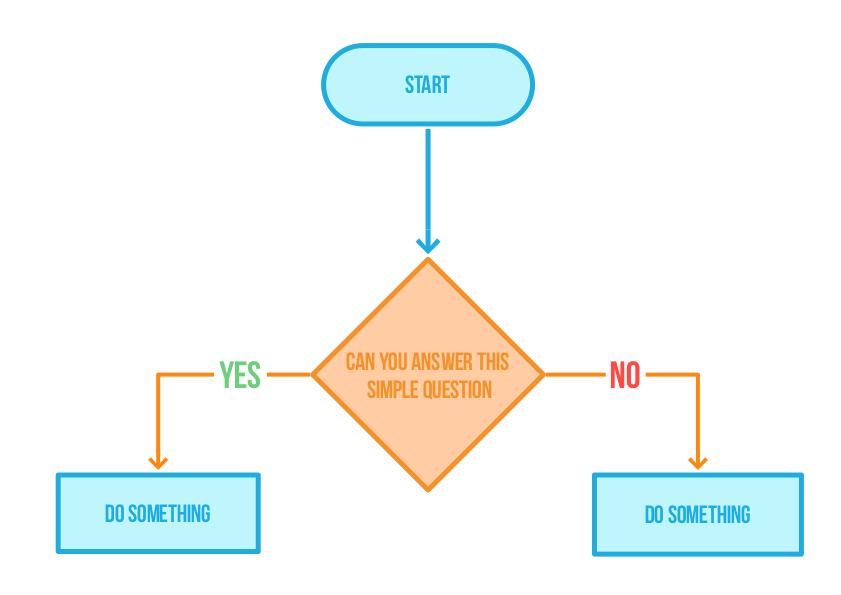
\includegraphics[scale=0.5]{figures/Flowchart}
    \caption{Caption for flowchart}
  	\medskip 
	\hspace*{15pt}\hbox{\scriptsize Credit: Acme company makes everything \url{https://acme.com/}}
    \label{FlowchartFigure}
\end{figure}

\subsection{Tables}

We can also do tables. Protip: use \url{https://www.tablesgenerator.com/} for generating tables.
\begin{table}[H]
\centering
\caption{Caption of table}
\label{TableLabel}
\begin{tabular}{|l|l|l|}
\hline
Title1 & Title2 & Title3 \\ \hline
data1  & data2  & data3  \\ \hline
\end{tabular}
\end{table}

\subsection{}

% Include more chapters as required.
%%=========================================
\renewcommand{\glossarypreamble}{\footnotesize}
\printglossary[style=super, type=\glsdefaulttype] \let\cleardoublepage\clearpage
\printglossary[style=super, type=\acronymtype]

%\bibliographystyle{plainnat}  %Set the type of bib you want to use in the text.

\printbibliography[heading=bibintoc]
\clearpage
% Include more appendices as required.
%%=========================================
%\clearpage
%\DeclareRobustCommand{\VAN}[3]{#3}
%\addcontentsline{toc}{chapter}{Bibliography}
%\bibliographystyle{generators/myplainnat}
%\bibliography{generators/refs}
%\appendix
\titleformat{\chapter}[hang]
  {\normalfont\large\bfseries}% <- font for label "Appendix A", default \huge
  {\thechapter}
  {20pt}
  {\large}% <- font for title, default \Huge
\titlespacing*{\chapter}{0pt}{0pt}{40pt}


\renewcommand\appendixpage{\vspace*{0.5cm}\thispagestyle{empty}\mbox{}\begin{flushleft}\Huge\bfseries\addappheadtotoc\appendixpagename\mbox{}\end{flushleft}\vspace*{1cm}}
\renewcommand{\cleardoublepage}{}
\renewcommand{\clearpage}{}
\begin{appendices}
\chapter{Generated code from Protocol buffers}

\begin{lstlisting}[caption={Source code of something},label=Listing]
System.out.println("Hello Mars");
\end{lstlisting}
\end{appendices}
\end{document}
